\section{Introduction}

\begin{figure*}[t]
\begin{center}
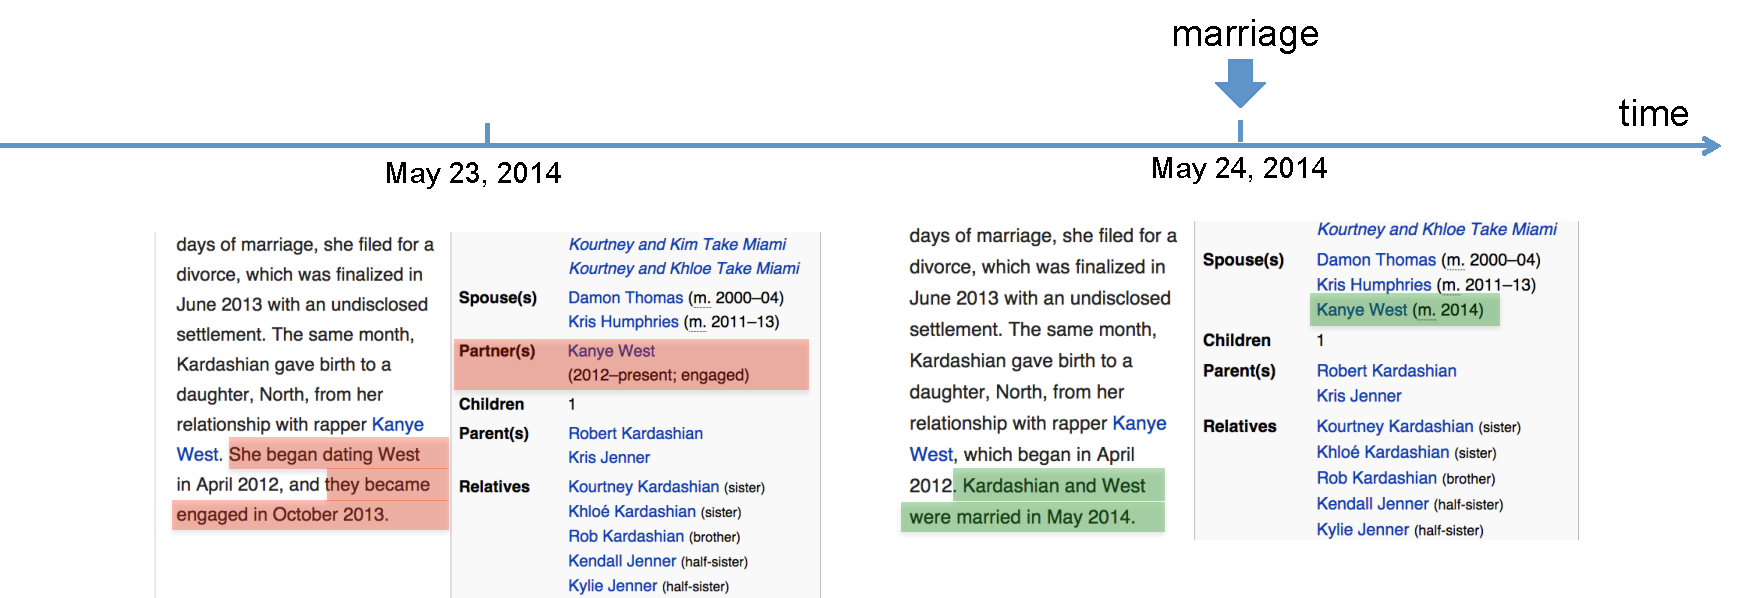
\includegraphics[width=14cm,keepaspectratio=true]{figures/motivation.pdf}
\caption{\label{fig:motivation} A snapshot of Kim Kardashian's Wikipedia revision history, highlighting text and infobox changes. In red (and green) are the difference between the page on 05/23/2014 and 05/24/2014: things that are deleted from (and resp. added to) the page.}
\end{center}
\end{figure*}

In recent years there has been a lot of research on extracting relational facts between entities and storing them in knowledge bases (KBs). These knowledge bases such as YAGO (which extract facts from Wikipedia infoboxes \cite{suchanek2007yago}) or NELL (which extracts facts from any Web text \cite{carlson2010toward,fader2011identifying}) are generally static. They are not updated as the Web changes when in reality new facts arise while others cease to be valid%or change over time
. One approach towards real-time population of KBs is to extract facts from dynamic content of the web such as news \cite{nakashole2012real}. This paper proposes a \textit{shift} of focus from doing KB updates by extracting facts in text to doing them by identifying state changes brought about by verbs in text. 

The benefit of such shift is multi-fold: (1) Detecting state change to an entity in text can be used to infer and update the entity's fact and its temporal scope in KB \cite{wijayactp}. (2) Learning state changes brought about by verbs can pave ways to learning the pre- and post-conditions of state-changing verbs: the entry condition (in terms of KB facts) that must be true for an event expressed by the verb to take place, and the exit condition (in terms of KB facts) that will be true after the event occurs. Such pre- and post-conditions can be useful for (a) learning event sequences %such as scripts \cite{schank2013scripts}, which can be modeled
as a collection of verbs chained together by pre- and post-condition of their shared entities, (b) for inferring cascading effect of an event via the pre- and post-condition of shared entities in an event sequence, or (c) for inferring unknown states of entities from the verbs they participate in.  

In this paper, we propose to learn state changes brought about by verbs using Wikipedia revision histories. Our assumption is that when a state-changing event happens to an entity e.g., a marriage, its Wikipedia infobox: a structured document that contains a set of facts (attribute-value pairs) of the entity is updated e.g., by the addition of a new \textsc{spouse} value. At the same time, texts that contain verbs that express the event e.g., \textit{wed} may be added to the entity's Wikipedia page (see an example in Figure \ref{fig:motivation}). Wikipedia revisions over many entities can act as distantly supervised data for mapping text and infobox changes that relate to events. However, Wikipedia revisions are \textit{noisy}: there is no guarantee that only the infobox slots related to a particular event will be updated. For example, when an event such as death happens, slots regarding birth e.g., \textit{birthdate}, \textit{birthplace}, may also be updated. To alleviate the effect of such, we leverage constraints between slots e.g., that \textit{deathdate} is mutually exclusive with \textit{birthdate} or that \textit{birthdate} is simultaneously updated with \textit{birthplace}, to effectively learn infobox changes that relate to a particular event-expressing verb. 

Our contribution is the construction and use of an interesting, distantly labeled, dataset from Wikipedia revisions for learning about verbs and state changes, and the learned resource of verbs effective for identifying state changes \footnote[1]{We make our dataset and verbs resource available here: http://.../verbs.html}.